\documentclass[8pt]{article}
\usepackage{blindtext}
\usepackage{listings}
\usepackage{graphicx}
\usepackage[a4paper, total={6in, 8in}]{geometry}

\title{Is Florida Getting Warmer}

\begin{document}
    \section{The interperation of whether Florida getting warmer or not}
    \begin{lstlisting}[language=R]
        #after load the data file, take the data into sets
        temp<- c(ats$Temp)
        year<- c(ats$Year)
        #observed coorelation between temperature and year
        Oricor<- cor(temp, year, method = "pearson")
        Oricor

        #using 5000 generation to simulate random situation
        nreps<-5000
        T.random<-numeric(nreps)
            
        #in each generation, calculate the correlation between two factors
        for (i in 1:nreps) {
            Y <- year
            X <- sample(temp, 100, replace = FALSE)   
            T.random[i] <-cor(X,Y)
        }
        #calculate the similar situation like observed one in the 
        #randon simulation
        prob <- length(T.random[T.random >= Oricor])/nreps
        #histgram the distribution of random one correlation
        hist(r.random, breaks = 50, main =  expression(paste(
            "Distribution around ",rho, "= 0")), 
            xlab = "correlation from randomized samples")
        \end{lstlisting}
    
    The code 'prob' showing nearly 0 possibility randomized temperature influence.
    Although the observed temperature is during a successive time-points, the comparison 
    between it and random time correlation showing that they have significant different.
    Thus, the 0.53 correlation inidcate the temperature has significant correlation with the years,
    which further indicate that Florida is getting warmer through the years. In addition, the
    graph below also showing the observed one is different with the random calculating one.
    
    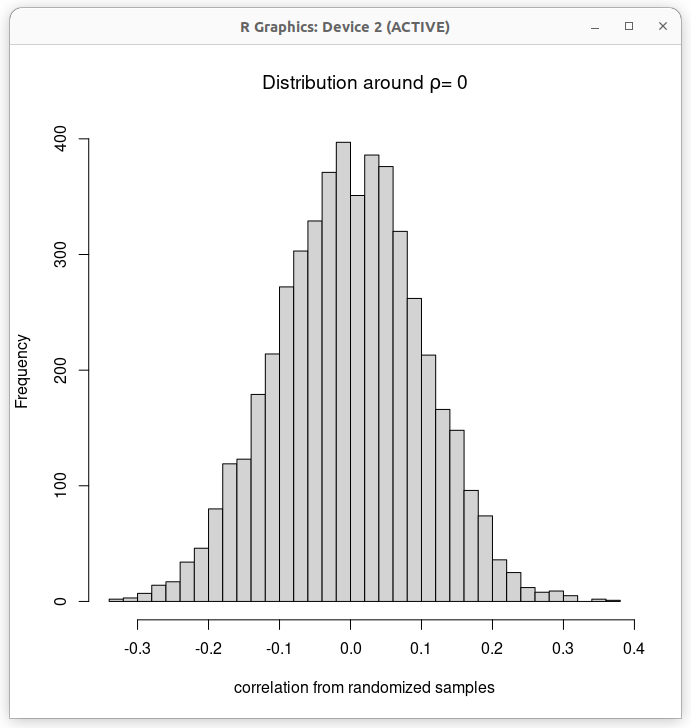
\includegraphics[width=\textwidth]{distribution around T}
    
    This graphic showing that the observed correlation is larger than 0.5 which is nearly tend to 0.

\end{document}








